\documentclass[a4paper, 11pt, nofootinbib]{article}

\setcounter{tocdepth}{3}
\setcounter{secnumdepth}{3}
\usepackage{amsmath}
\usepackage{comment} % enables the use of multi-line comments (\ifx \fi) 
\usepackage{lipsum} %This package just generates Lorem Ipsum filler text. 
\usepackage{fullpage} % changes the margin
\usepackage[utf8]{inputenc}
\usepackage{gensymb}
\usepackage{graphicx}
\usepackage{booktabs}% http://ctan.org/pkg/booktabs
\usepackage{makecell}
\usepackage{tabularx}
\usepackage[table]{xcolor}
\usepackage{array}
\usepackage{wrapfig}
\usepackage{subcaption}
\usepackage{csquotes}
\usepackage{lscape}
\usepackage{afterpage}
\usepackage{geometry}
\usepackage{listings}
\usepackage{xcolor}
\usepackage{ulem}

\geometry{a4paper, margin=1in}

\renewcommand{\figurename}{Abb.}
\newcommand{\code}[1]{\texttt{#1}}
\renewcommand{\contentsname}{Inhalt}
\renewcommand{\listfigurename}{Abbildungsverzeichnis}


\begin{document}
\title{Zusammenfassung Information Security FS2018}
\author{Alex Neher}
\maketitle

\tableofcontents
\newpage
\listoffigures
\newpage

\graphicspath{{./Pictures/}}

\section{Teil Pouly}
\subsection{Nach welchen Kriterien lassen sich Hacker und ihre Opfer klassifizieren?}

\paragraph{Hacker}\mbox{}\\

\noindent • Hacktivisten\\
• Cyberterroristen\\
• Staatliche Organisationen\\
• Skript Kiddies\\
• Organisiertes Verbrechen\\
• Wissenschaftler / Krypto-Analytiker\\

\paragraph{Opfer}\mbox{}\\

\noindent • Einzelpersonen (gezielt)\\
• Einzelpersonen (zufaellig)\\
• Die grosse Masse (zufaellig)\\
• Organisationen / Firmen (gezielt)\\

\subsection{Wleche Angriffstrategien werden typischerweise gegen welche Opfer eingesetzt?}

\begin{itemize}
	\item Einzelpersonen (gezielt)
		\subitem Identitätsdiebstahl
		\subitem Informationsdiebstahl
		\subitem Diskreditierung
	\item Einzelpersonen (zufällig)
		\subitem Phishing
		\subitem Skimming
	\item Die grosse Masse (zufällig)
		\subitem Viren-Angriffe auf bestimmte Betriebssysteme
	\item Firmen und Organisationen (gezielt)
		\subitem DDoS
\end{itemize}

\subsection{Beschreiben Sie zwei unterschiedliche Geschäftsmodelle von Hacking Organisationen}
\begin{itemize}
	\item Erpressung
	\item DDoS As a Service
\end{itemize}

\subsection{Was versteht man unter Identitätsdiebstahl?}
1. Ein Hacker stielt das E-Mail Passwort seines Vorgesetzten.\\
2. Ein Hacker stielt das Login Passwort zum PC eines Mitarbeiters.\\
3. Ein Hacker stielt ein Facebook Passwort.\\

In den USA ist Identitaetsdiebstahl ein grosses Problem, weil es dort – anders
als in der Schweiz – mit der Sozialversicherungsnummer ein personenbezogenes
Merkmal gibt, das hinreichend ist, um Steuern zurueckzufordern und Kreditkar-
tenvertraege abzuschliessen. [...] Allein 2011 belief sich der finanzielle Schaden
infolge von Identitaetsdiebstahl auf 3.6 Mrd. USD. NZZ, 20.01.2014

\subsection{Beschreiben Sie mögliche Konsequenzen von Identitätsdiebstahl für die Opfer}
• Finanzielle Folgen (Bestellungen auf meinen Namen etc)\\
• Rechtliche Folgen (Kinderpornografie etc)\\
• Gesellschaftliche Folgen (Postings von meinem FB Account)\\

\newpage

\subsection{Analysieren Sie die Authentifikationsmethoden 1-4 auf Stärken und Schwächen}

\begin{figure}[htb]
	\centering
	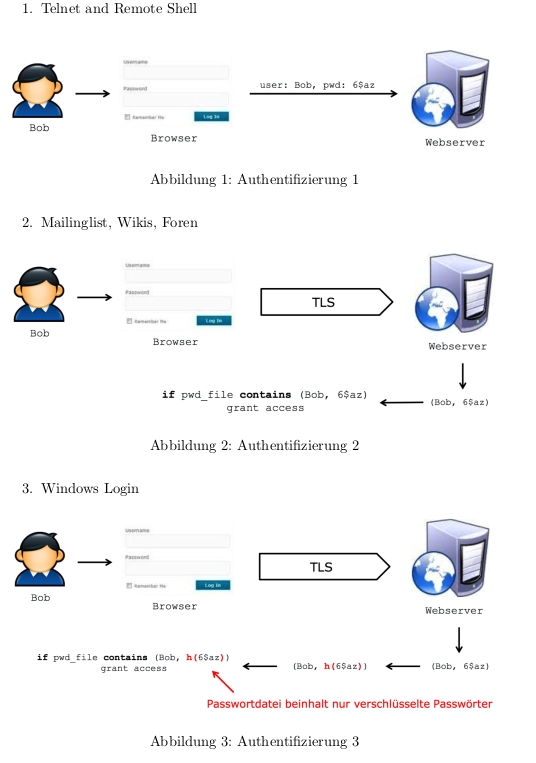
\includegraphics[keepaspectratio=true,height=27\baselineskip]{authentification.jpg}
\end{figure}
\begin{figure}[htb]
	\centering
	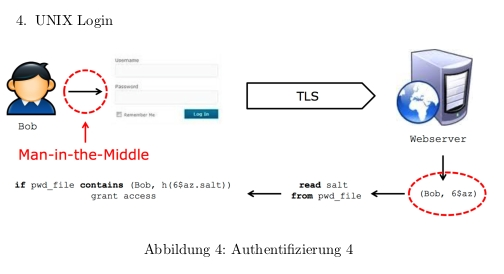
\includegraphics[keepaspectratio=true,height=9\baselineskip]{authentification_2.jpg}
\end{figure}

\newpage

\subsection{Wie schützen Betriebssysteme typischerweise unsere Identitäten und wie kann dieser Schutz mit Maschinenzugriff ausgehebelt werden?}
\paragraph{Windows}\mbox{}\\
Windows Betriebssysteme (seit NT) speichern Passwortinformationen in der Re-
gistry Datei Security Account Manager (SAM). Windows Kernel sichert SAM,
so dass Datei nicht kopiert werden kann.

So geht es trotzdem...
Dumping File Sectors directly from Disk using Logical Offsets $\rightarrow$ Cain\\
Wenn SysKey aktiviert ist, verschluesselt Windows die SAM Datei partiell.\\
Wenn SysKey aktiviert ist, holt bkhive den Schluessel aus der Registry.\\

\begin{figure}[htb]
	\centering
	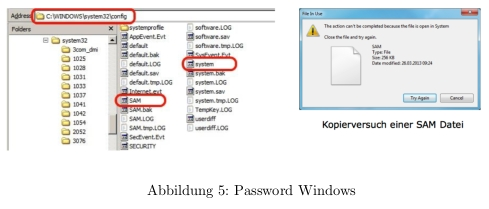
\includegraphics[keepaspectratio=true,height=12\baselineskip]{SAM_Windows.jpg}
\end{figure}

\paragraph{Linux}\mbox{}\\
Unix Betriebssysteme (seit 1990) speichern Passwortinformationen in Shadow
Dateien. Nur Superuser koennen diese Dateien lesen.

\begin{figure}[htb]
	\centering
	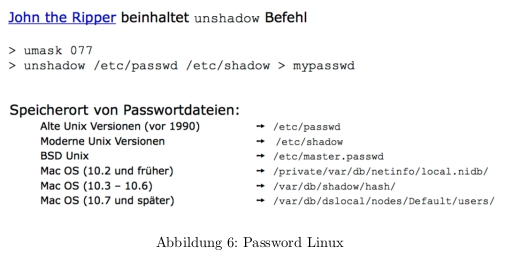
\includegraphics[keepaspectratio=true,height=12\baselineskip]{password_linux.jpg}
\end{figure}

\paragraph{Fazit}\mbox{}\\
• In Klartext gespeicherte (z.B. FileZilla) oder gecachte (z.B. Windows-
Domaenen Anmeldung) Passwoerter koennen mit Maschinenzugriff leicht
geklaut werden.\\
• Betriebssysteme schuetzen Passwortdateien, jedoch kann der Schutz leicht
umgangen werden.\\
• Anwendungsprogramme und Betriebssysteme verschluesseln Passwoerter
bevor sie in einer Passwortdatei abgelegt werden.\\

\subsection{WelcheAngriffsstrategien auf gestohlene Passwort-Hashes hat ein Hacker zur Verfügung?}

\begin{enumerate}
	\item Passwort-Hashfunktion knacken
	\item Brute-Force Attacke
		\subitem Alle möglichen Kombinationen werden systematisch durchprobiert
		\subitem Jedes mögliche Passwort wird verschlüsselt und in der Passwort-Datei gesucht
		\subitem Irgendeinmal wird jedes System so geknackt $\rightarrow$ Vollständige Methode
	\item Dictionary Attacke
		\subitem Nur Wörter aus einem vorgegebenen Wörterbuch werden durchprobiert
		\subitem Beruht auf der Annahme, dass sinnvolle Wörter als Passwort verwendet werden, oder dass das Passwort auf einem Algorithmus beruht (z.B. Palindrom)
		\subitem Knackt das System nur, falls sich das Passwort im Wörterbuch befindet $\rightarrow$ Unvollständige Methode
	\item Lookup Tabelle
		\subitem Wörterbuch mit Wort und dazugehörigem Hash
		\subitem Wörterbuch mit 1 Million Wörtern verlangt 1 Million Hashberechnungen
		\subitem Es muss nun nur noch nach dem Hashwert gesucht werden
		\subitem Es wird mehr Memory benötigt, dafür wird Zeit gespart
		\subitem Gleich wi<e Dictionary-Attack: Knackt nur Passwörter in der Tabelle $\rightarrow$ Unvollständige Methode
\end{enumerate}

\subsection{Sie können den Aufwand von Brute-Force Attacken vorausbereichnen}
Passwörter bestehen aus alphanumerischen Symbolen (a-z,A-Z,0-9) und 8 möglichen Zusatzzeichen ( 26 + 26 + 10 + 8 = 70 Zeichen). Das CMS Joomla verschlüsselt die Passwörter mit MD5. Angenommen, man verwendet die Software oclHashcat und 2 GPUs mit 880Mhz getaktet und 1250Mhz getaktete RAM. Die Benchmark zeigt 23083.9 M/s an $\rightarrow$ ca. $23 * 10^{9}$ Hashes/s

\paragraph{Passwort der Länge 7}\mbox{}\\
\begin{equation}
\dfrac{70^{7}  Hashes}{23*10^{9}   Hashes/sek} = 358sek = 5.96 Min
\end{equation} 

\paragraph{Passwort der Länge 9}\mbox{}\\
\begin{equation}
\dfrac{70^{9}  Hashes}{23*10^{9}   Hashes/sek} = 1754504sek = 487.3h = 20.3 Tage
\end{equation} 

\paragraph{Passwort der Länge 11}\mbox{}\\
\begin{equation}
\dfrac{70^{11}  Hashes}{23*10^{9}   Hashes/sek} = 8597072795sek  = 99503 TAge = 272.6 Jahre
\end{equation} 

\subsection{Nennen Sie den Unterschied zwischen Dictionaries und Lookup-Tabellen}
Lookup-Tabellen sind vorgefertigte Tabellen, die einen Hashwert und das dazugehörige Klartext-Passwort enthalten. Die Hashes sind bereits berechnet. Man muss nur noch anhand des Hashes, welches z.B. im shadows File gefunden werden kann, das Passwort heraussuchen. 

Ein Dictionary ist im Gegensatz zur Lookup-Tabelle nur eine Sammlung von möglichen Passwörtern im Klartext. Man kann z.B. einen einfachen Duden als Dictionary verwenden. Anschliessend wird für jedes Wort den Hash berechnet und mit dem gewünschten Hash verglichen.

\subsection{Sie können die Funktionsweise von Rainbow-Tables anhand eines Beispiels erklären}


\section{Teil Portmann}

\section{Teil Bürgler}

\end{document}